% =============================================================================
% paper_marco2c/main.tex
% Disentangling Timing from Architecture in Recurrent Spiking Networks:
% A Characterization on Spiking Heidelberg Digits
% Author: Luis Roberto Pinho da Silva Junior (Independent research)
%
% Status: LaTeX consolidado no kickoff. 6 seções + abstract + 3 figuras + refs.
% Compilar via Overleaf (upload main.tex + refs.bib + figs/) ou pdflatex+bibtex local.
% =============================================================================

\documentclass[11pt]{article}
\usepackage[margin=1in]{geometry}
\usepackage[utf8]{inputenc}
\usepackage{amsmath,amssymb,amsthm}
\usepackage{graphicx}
\usepackage{booktabs}
\usepackage{hyperref}
\usepackage{xcolor}
\usepackage{authblk}
\usepackage[round]{natbib}
\bibliographystyle{plainnat}

\hypersetup{colorlinks=true, citecolor=blue, linkcolor=black, urlcolor=blue}

\title{Disentangling Timing from Architecture in Recurrent Spiking Networks:\\A Characterization on Spiking Heidelberg Digits}
\author[1]{Luis Roberto Pinho da Silva Junior}
\affil[1]{Independent research \\ \url{https://github.com/luisroberto0/project-hebb}}
\date{2026}

\begin{document}
\maketitle

\begin{abstract}
Recurrent spiking neural networks (SNNs) are routinely reported to exploit temporal structure, but the measured advantage over a non-temporal baseline conflates two effects: information genuinely carried by spike \emph{timing}, and architectural differences (LIF dynamics, normalization) unrelated to timing. We characterize a recurrent LIF network on the Spiking Heidelberg Digits (SHD) dataset, separating the two as far as a resolution sweep allows. The recurrent SNN reaches 71.27\% versus 51.56\% for a timing-blind baseline (a per-channel spike histogram followed by an MLP), a gap of 19.7 percentage points. By sweeping the temporal resolution, we \textbf{bound the genuine timing contribution at $\sim$+10 p.p.} (the same network as it goes from 1 to 100 time bins) and attribute $\sim$+9.5 p.p.\ to architecture (a single-bin SNN still beats the MLP); we flag that the single-bin anchor also disables the recurrent pathway, so the timing figure is an upper bound that bundles timing with recurrence becoming operative. The network recovers 50.68\% from onset timing alone (one spike per channel). Temporal k-WTA sparsity is tolerated up to 75\% at a cost of 1.50 p.p.---close to the 1.45 p.p.\ tolerance we reported for \emph{spatial} k-WTA in unpublished companion work, a suggestive parallel we do not over-read. The effect is dataset-specific: on the harder Spiking Speech Commands it is weak and training-dependent ($\sim$+4--5 p.p., single seed). Crucially, a \emph{non-spiking} GRU on the same input reaches 79.64\%, exceeding the SNN by 10.5 p.p.: the timing contribution is generic to recurrence, not spiking-specific, and the SNN is not a competitive way to exploit it. We claim no superiority for spiking networks and no new mechanism; we quantify, with controls, how much timing helps, by what, and where its benefit ends.
\end{abstract}

% =============================================================================
\section{Introduction}
\label{sec:intro}

Spiking neural networks (SNNs) process information as discrete events in time, and a recurring claim is that they exploit the \emph{timing} of those events---that the moment a unit fires, not merely whether it fires, carries information~\citep{maass1997networks}. On temporal benchmarks such as the Spiking Heidelberg Digits (SHD)~\citep{cramer2020heidelberg}, recurrent SNNs reach accuracies well above non-temporal baselines, and this gap is often attributed to timing. We argue that the attribution is, as usually measured, confounded.

The advantage of a recurrent SNN over a non-temporal baseline mixes two distinct effects. The first is information genuinely carried by spike timing: if the same network is given finer temporal resolution and improves, that improvement is attributable to timing. The second is architectural: an SNN uses LIF dynamics, often batch normalization, and a different readout than a plain multilayer perceptron (MLP), and these differences can move accuracy regardless of any temporal structure. A network given only a single time step---which destroys all timing---can still differ from an MLP for purely architectural reasons. Reporting the raw gap therefore \emph{overstates} how much timing helps.

This paper characterizes a recurrent LIF network on SHD with that confound controlled. Our baseline is deliberately \emph{timing-blind}: we sum each input channel's spikes over the entire trial (a per-channel histogram) and classify the resulting vector with an MLP. This preserves \emph{which} channels fired---the average spectral content---while destroying \emph{when}. The difference between the recurrent SNN and this baseline isolates the contribution of timing, controlling for the spectral information both representations share.

\textbf{Main findings.} (i) On SHD (5 seeds, bootstrap 95\% CIs), the recurrent SNN reaches 71.27\% versus 51.56\% for the timing-blind baseline---a raw gap of 19.7 p.p. (ii) Sweeping the number of time bins from 1 to 100 shows accuracy rising monotonically; the \emph{same} network improves by 10.18 p.p.\ as resolution increases, an \textbf{upper bound on the genuine timing contribution} (the single-bin anchor also disables recurrence, so this gain bundles timing with the recurrent pathway becoming operative; see \S\ref{subsec:bins}). The residual (a single-bin SNN still beats the MLP by $\sim$9.5 p.p.) is architectural, not temporal. (iii) Under latency coding (one spike per channel, at the time of its first event), the network still reaches 50.68\%---far above chance and above a presence-only baseline---exploiting information beyond binary channel presence, consistent with its using onset timing. (iv) Temporal k-WTA, which keeps only the $k$ most-active hidden units per time step, tolerates 75\% sparsity at a cost of 1.50 p.p.; this is close to the 1.45 p.p.\ tolerance of \emph{spatial} k-WTA we reported in unpublished companion work~\citep{pinho2026kwta}, and collapses only under extreme ($>$96\%) sparsity. (v) The effect is dataset-specific: on the larger, harder Spiking Speech Commands the timing margin is weak and training-dependent ($+5.2$ p.p.\ at 35 epochs, eroding to $+3.95$ at 60; single seed). (vi) Most consequentially, a \emph{non-spiking} GRU on the same input reaches 79.64\%, exceeding the recurrent SNN by 10.5 p.p.: the timing contribution is generic to recurrence, not spiking-specific, and the SNN is not a competitive way to exploit it.

The contribution is characterizational, not methodological: a controlled (if first-order) decomposition of the timing/architecture confound, corroborated by independent probes (latency coding, the resolution curve), a quantitative temporal k-WTA tolerance curve, and a measured generalization limit. We make no claim of superiority over conventional methods---a convolutional or transformer model on a spectrogram exceeds 90\% on these benchmarks, well above the SNN. We make no claim of a new learning mechanism: training is by surrogate-gradient backpropagation. The value is a controlled, honest measurement of how much spike timing contributes, and where that contribution ends.

% =============================================================================
\section{Background}
\label{sec:background}

\subsection{Spiking Networks and Surrogate-Gradient Training}
A spiking neuron integrates input over time and emits a discrete spike when its membrane potential crosses a threshold, after which the potential resets. We use the leaky integrate-and-fire (LIF) neuron: $u_t = \beta u_{t-1} + I_t$, with a spike when $u_t > \vartheta$ and a reset thereafter. The spike function is non-differentiable, so end-to-end training uses a \emph{surrogate gradient}---a smooth function substituted for the derivative of the threshold during backpropagation through time~\citep{neftci2019surrogate}. We use the fast-sigmoid surrogate. We emphasize at the outset that surrogate-gradient training \emph{is} backpropagation; this work characterizes what the temporal dynamics compute, not a backprop-free learning rule.

A recurrent SNN adds lateral connections in the hidden layer, so the state at one time step feeds the next, giving the network an explicit mechanism to integrate information across time. We contrast a feedforward SNN (temporal input, no recurrence) and a recurrent SNN against a timing-blind MLP, and---to test whether any advantage is spiking-specific---against a non-spiking recurrent network (a GRU, \S\ref{subsec:gru}).

\subsection{The Spiking Heidelberg Datasets}
The Spiking Heidelberg Digits (SHD) and Spiking Speech Commands (SSC) datasets~\citep{cramer2020heidelberg} convert spoken audio into spike trains through a model of the inner ear: each utterance becomes events across 700 input channels (frequency-like cochlear bands) over roughly one second. SHD contains spoken digits 0--9 in English and German (20 classes, $\sim$10{,}000 samples, speaker-held-out test split). SSC is larger and harder: 35 command words, $\sim$100{,}000 samples. Because the information is intrinsically temporal, these benchmarks are standard for evaluating whether a model exploits timing. Reported recurrent-SNN accuracies on SHD lie in the 70--83\% range; feedforward SNNs are lower (48--66\%).

\subsection{k-WTA and Sparse Coding}
The $k$-winner-take-all (k-WTA) operation keeps the $k$ largest entries of an activation vector and zeros the rest~\citep{maass2000computational}. It has direct biological motivation---cortical activity is sparse---and appears across cortex-inspired models. In a companion study on Prototypical Networks~\citep{pinho2026kwta}, k-WTA applied to a \emph{spatial} embedding was shown to be tolerated in-domain: 75\% sparsity cost only 1.45 percentage points on Omniglot few-shot classification. Here we apply k-WTA along the \emph{temporal} axis (limiting how many hidden units may fire per time step) and ask whether the same tolerance holds. The parallel matters: it tests whether the compatibility of k-WTA sparsity with a trained representation is a property of the axis (spatial) or a more general phenomenon.

\subsection{Why a Timing-Blind Baseline}
To isolate the contribution of timing we need a baseline that has access to everything \emph{except} timing. We use the per-channel spike histogram: for each of the 700 channels, the total number of spikes over the trial, classified by an MLP. This representation preserves \emph{which} channels were active and how much---the average spectral envelope, which is itself discriminative for speech---while discarding \emph{when} each spike occurred. The gap between a temporal model and this baseline therefore measures the value of timing \emph{controlling for} the spectral information both share. This is a stronger control than comparing against chance: on SHD the timing-blind baseline already reaches $\sim$51\%, far above the 5\% chance level, precisely because the spectral envelope carries much of the signal. What the SNN must add, to justify its temporal machinery, is information that survives only in the timing.

% =============================================================================
\section{Method}
\label{sec:method}

\subsection{Models}
All three models map a sample to logits over the classes; they differ only in how they use time.
\textbf{Timing-blind baseline (BlindMLP).} The input spike tensor $(T, 700)$ is summed over time to a 700-dimensional per-channel histogram, then passed through an MLP ($700 \to 256 \to C$, ReLU). It has no access to temporal order.
\textbf{Feedforward SNN.} A LIF layer ($700 \to 256$) processes the input one time step at a time, followed by an integrating readout ($256 \to C$); no recurrence.
\textbf{Recurrent SNN.} As above, with an all-to-all recurrent connection in the hidden layer: $I_t = \mathrm{BN}(W_{\text{in}} x_t) + W_{\text{rec}} s_{t-1}$, where $s_{t-1}$ is the previous hidden spike vector. This is the model that can integrate timing across the trial.

Hidden size 256, LIF decay $\beta = 0.9$, fast-sigmoid surrogate. The readout is an \emph{integrator}: logits are the sum over time of a linear projection of the hidden spikes, $\sum_t W_{\text{out}} s_t$. We found a spiking output layer trained poorly (the output rarely fired, starving the loss of gradient); the linear integrating readout gives continuous, well-conditioned logits.

\subsection{A Reproducible Training Detail: BatchNorm Statistics}
Without normalization the input current sat far below threshold (hidden firing rate $\sim$3.7\%) and training was slow. Adding BatchNorm on the hidden pre-activation fixed the scale, but introduced a subtle failure: with default running statistics, accuracy trained to $>$70\% yet \emph{tested} near chance (13\%). The cause is that a single BatchNorm, applied at every one of the 100 time steps, accumulates running mean/variance that mix all time steps; at evaluation those pooled statistics are wrong for any individual step. Setting \texttt{track\_running\_stats=False} (using batch statistics at test time as well) resolves it, lifting test accuracy from 13\% to 71\%. We report this because it is an easy, silent trap when batch-normalizing a per-time-step SNN.

\subsection{Input Encodings}
\textbf{Rate.} Each $(T,700)$ tensor counts spikes per (time-bin, channel). Time is binned into $T$ bins (default $T=100$) over the $\sim$1.4\,s trial.
\textbf{Latency (time-to-first-spike).} For each channel, a single spike is placed in the bin of its \emph{first} event; later spikes are discarded. This keeps only onset timing (one spike per active channel) and lets us test whether onset timing alone is informative.

\subsection{Temporal k-WTA}
At each time step, after computing hidden spikes, we keep only the $k$ units with the largest membrane potential and zero the rest, enforcing at most $k$ active hidden spikes per step. Sweeping $k \in \{128, 64, 32, 16, 8, 4\}$ over a hidden size of 256 spans 50\%--98.4\% temporal sparsity.

\subsection{Datasets and Evaluation}
We use the official SHD train/test split (speaker-held-out test). Spikes are read from the published HDF5 files. The main result uses 5 seeds with 95\% bootstrap confidence intervals over the per-seed accuracies. The resolution, latency, and k-WTA characterizations use 3 seeds. For the SSC generalization (Section~\ref{subsec:ssc}) we train on the full $\sim$75{,}000-sample training set via lazy HDF5 loading, on a \emph{single seed} (so without a CI), which we weigh accordingly. Training uses Adam ($10^{-3}$) and cross-entropy on the integrated logits. All experiments run on a single RTX 4070 laptop GPU; we note that the recurrent loop over 100 time steps leaves the GPU largely idle, a practical signature of how poorly the sequential-temporal computation maps onto dense parallel hardware.

% =============================================================================
\section{Experiments}
\label{sec:experiments}

\subsection{Main Result on SHD}
\label{subsec:main}
Table~\ref{tab:shd} reports 5-seed accuracy on the SHD test split.

\begin{table}[tbp]
\centering\small
\caption{SHD test accuracy (5 seeds). $\pm$ is the standard deviation across seeds; brackets are 95\% bootstrap CIs (legitimately asymmetric, so not centered on the mean). Chance is 5\%.}
\label{tab:shd}
\begin{tabular}{lrr}
\toprule
Model & Accuracy & 95\% CI \\
\midrule
Timing-blind baseline (histogram + MLP) & 51.56\% $\pm$0.77 & [50.78, 52.09] \\
SNN feedforward                         & 61.02\% $\pm$0.85 & [60.27, 61.77] \\
SNN recurrent                           & 71.27\% $\pm$0.45 & [70.91, 71.70] \\
\bottomrule
\end{tabular}
\end{table}

The recurrent SNN exceeds the timing-blind baseline by \textbf{19.71 p.p.}\ and exceeds the feedforward SNN by 10.26 p.p.\ (Figure~\ref{fig:conditions}); the three per-condition CIs do not overlap. Taken at face value, this 19.7 p.p.\ gap is the ``timing advantage.'' The rest of this section shows that roughly half of it is not timing.

\begin{figure}[tbp]
\centering
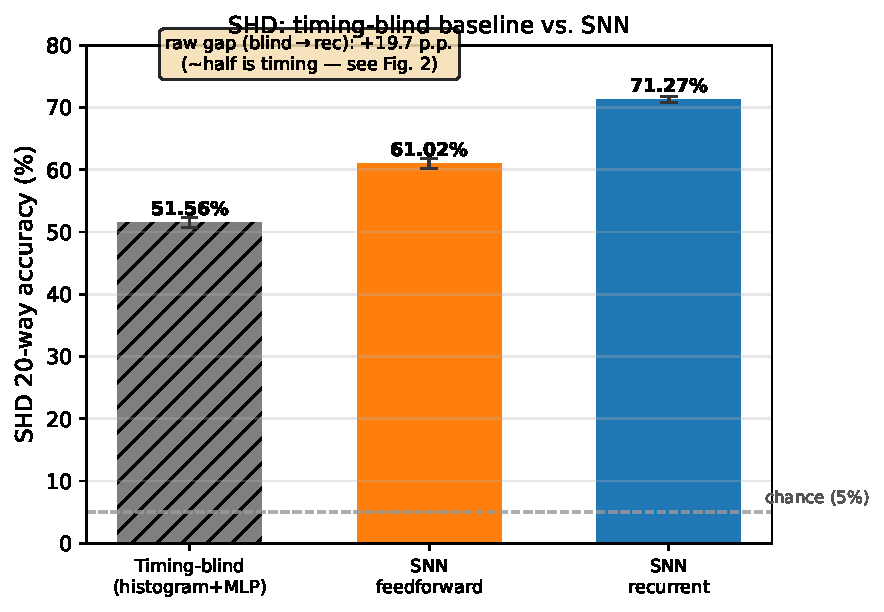
\includegraphics[width=0.72\linewidth]{figs/fig1_shd_conditions.pdf}
\caption{SHD test accuracy for the three conditions (5 seeds, 95\% CIs). The raw gap between the timing-blind baseline and the recurrent SNN is 19.7 p.p.; Section~\ref{subsec:bins} shows about half is architectural rather than temporal.}
\label{fig:conditions}
\end{figure}

\subsection{Disentangling Timing from Architecture}
\label{subsec:bins}
We sweep the number of time bins $T$ for the recurrent SNN, holding the weights and layers fixed. At $T=1$ the input collapses to the per-channel histogram---the same information the blind baseline sees. One consequence of this anchor must be stated plainly: at $T=1$ the recurrent term $W_{\text{rec}} s_{t-1}$ has no previous step to act on ($s_0 = 0$) and there is a single LIF step, so the $T=1$ network is effectively a single-step feedforward LIF+BN net---recurrence, the architecture's defining feature, is \emph{inert}. As $T$ grows, the same weights gain access to finer timing \emph{and} the recurrent/multi-step dynamics become operative; the sweep alone cannot separate these two.

\begin{table}[tbp]
\centering\small
\caption{Recurrent SNN accuracy vs.\ temporal resolution (3 seeds, 8 epochs---a lighter budget than the 5-seed, 15-epoch main result, hence the $T{=}100$ point sits $\sim$2 p.p.\ below the 71.27\% headline of Table~\ref{tab:shd}). Timing-blind baseline: 49.41\%.}
\label{tab:bins}
\begin{tabular}{rrr}
\toprule
Time bins & Accuracy & vs.\ baseline \\
\midrule
1   & 58.92\% & +9.51 \\
4   & 63.06\% & +13.65 \\
16  & 67.29\% & +17.87 \\
32  & 68.45\% & +19.04 \\
100 & 69.10\% & +19.68 \\
\bottomrule
\end{tabular}
\end{table}

Accuracy rises monotonically with resolution (Table~\ref{tab:bins}, Figure~\ref{fig:resolution}); this gives a first-order decomposition. From $T=1$ to $T=100$ the same weights improve by \textbf{+10.18 p.p.}; we read this as an \emph{upper bound} on the genuine-timing contribution, because increasing $T$ also activates the recurrent and multi-step LIF dynamics that are inert at $T=1$ (and shifts the per-step normalization regime), none of which we separately control. The residual \textbf{+9.51 p.p.}\ at $T=1$ is the advantage of a single-step LIF+BN readout over the MLP on the same histogram---a feedforward, not recurrent, architecture. As a loose bound on the recurrence share, the feedforward-vs-recurrent gap at full resolution is +10.26 p.p.\ (Table~\ref{tab:shd}). The decomposition is computed on the 3-seed resolution sweep, whose total gap (19.68 p.p., baseline 49.41\%) reproduces the 5-seed headline (19.71 p.p.) to within 0.03 p.p.; of it, at most about half is genuine timing, so reporting the raw gap overstates the temporal contribution.

\begin{figure}[tbp]
\centering
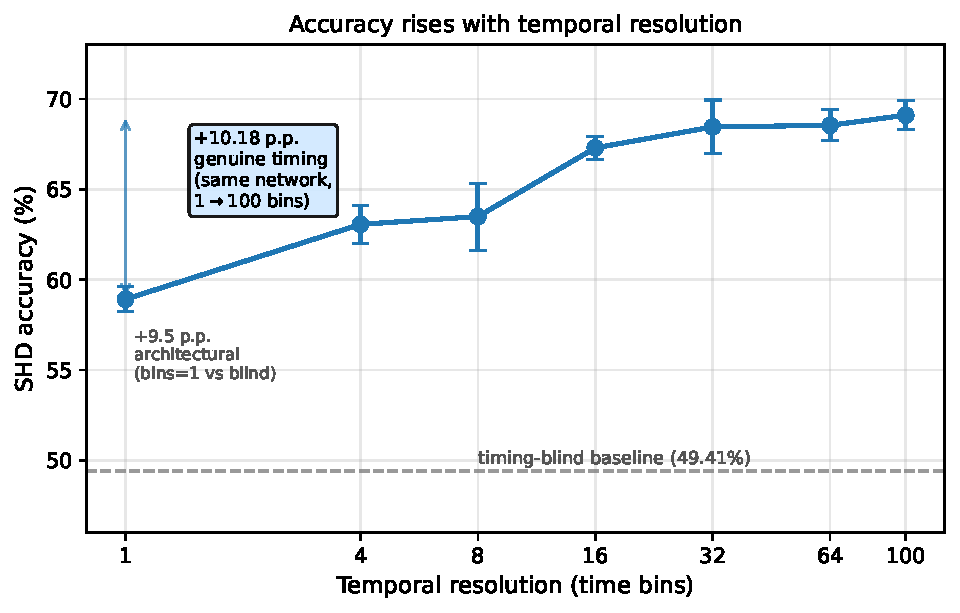
\includegraphics[width=0.8\linewidth]{figs/fig2_resolution.pdf}
\caption{Recurrent SNN accuracy vs.\ temporal resolution. The same weights improve by +10.18 p.p.\ from 1 to 100 bins---an upper bound on the timing contribution, since recurrence is inert at $T{=}1$ (see text). The +9.5 p.p.\ at a single bin, over the timing-blind baseline, is the feedforward LIF+BN architecture.}
\label{fig:resolution}
\end{figure}

\subsection{Onset Timing Alone Is Informative}
\label{subsec:latency}
Under latency coding, each channel contributes a single spike at its first-event time (Table~\ref{tab:latency}).

\begin{table}[tbp]
\centering\small
\caption{Rate vs.\ latency coding (3 seeds).}
\label{tab:latency}
\begin{tabular}{lrr}
\toprule
Coding & Timing-blind & SNN recurrent \\
\midrule
rate    & 49.41\% & 69.10\% \\
latency & 23.51\% & 50.68\% \\
\bottomrule
\end{tabular}
\end{table}

With one spike per channel---pure onset timing---the recurrent SNN still reaches \textbf{50.68\%}, far above chance (5\%) and above the latency-coded blind baseline (23.51\%, which retains only binary channel presence and is therefore weak). This shows the network exploits information beyond binary channel presence, consistent with its using onset timing. At the same time, full rate coding (69.10\%) beats latency (50.68\%) by 18.4 p.p.: the complete spike count carries substantial information beyond the onset. Timing helps, but it is not the whole story.

\subsection{Temporal k-WTA Tolerance Parallels the Spatial Case}
\label{subsec:kwta}
We apply k-WTA per time step on the hidden layer (Table~\ref{tab:kwta}, Figure~\ref{fig:kwta}).

\begin{table}[tbp]
\centering\small
\caption{Recurrent SNN under temporal k-WTA (3 seeds). Hidden size 256.}
\label{tab:kwta}
\begin{tabular}{rrr}
\toprule
$k$ & Sparsity & Accuracy (vs.\ dense) \\
\midrule
dense & 0\%    & 69.10\% \\
128 & 50\%     & 69.60\% (+0.50) \\
64  & 75\%     & 67.59\% ($-$1.50) \\
32  & 87.5\%   & 62.71\% ($-$6.39) \\
16  & 93.8\%   & 55.54\% ($-$13.56) \\
8   & 96.9\%   & 48.98\% ($-$20.11) \\
4   & 98.4\%   & 42.64\% ($-$26.46) \\
\bottomrule
\end{tabular}
\end{table}

Temporal k-WTA is tolerated up to 75\% sparsity ($k=64$) at a cost of only \textbf{1.50 p.p.}---close to the 1.45 p.p.\ cost of 75\% \emph{spatial} k-WTA we reported in-domain for Prototypical Networks~\citep{pinho2026kwta}. (That figure is from our own unpublished companion work, on a different dataset, architecture, and task; the two costs coincide to one decimal but with no shared error model, so we read the agreement as a suggestive coincidence worth following up, not a matched effect.) Degradation accelerates past 87.5\% and collapses beyond 96\% ($k \le 8$), where accuracy returns to the timing-blind baseline: with too few active units per step, the temporal representation has insufficient capacity. This single temporal point, alongside the single spatial point, is \emph{consistent with}---but does not establish---k-WTA tolerance being axis-independent in-domain.

\begin{figure}[tbp]
\centering
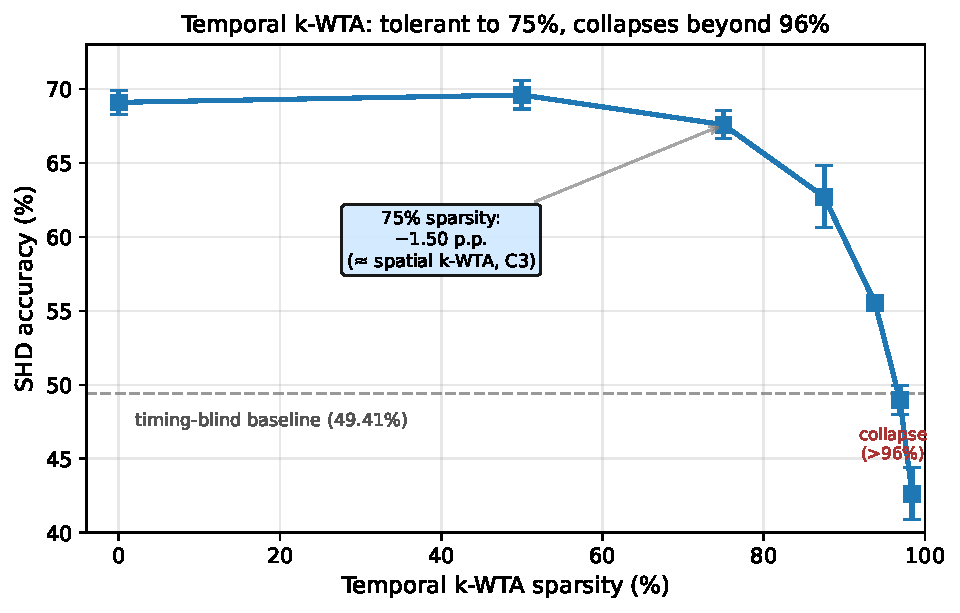
\includegraphics[width=0.8\linewidth]{figs/fig3_kwta_temporal.pdf}
\caption{Recurrent SNN under temporal k-WTA. Sparsity is tolerated to 75\% ($-$1.50 p.p., close to the spatial case) and collapses to the timing-blind baseline beyond 96\%.}
\label{fig:kwta}
\end{figure}

\subsection{Generalization to SSC Is Weak and Training-Dependent}
\label{subsec:ssc}
We repeat the main comparison on the harder SSC (35 classes; full $\sim$75k training set; \emph{single seed}, so without a CI). The recurrent SNN reaches 30.83\% versus 25.63\% for the blind baseline, a timing margin of \textbf{+5.20 p.p.} (35 epochs). Training longer (60 epochs) does not grow the margin---it falls to +3.95 p.p., with the SNN slightly overfitting. With a single seed at two epoch budgets the margin did not grow, which \emph{suggests but does not establish} a ceiling rather than undertraining (a 1.25 p.p.\ difference between single runs is within plausible seed noise). The timing effect therefore appears to \emph{generalize qualitatively} (positive on both datasets) but to be \emph{dataset-specific in magnitude}: strong on SHD ($\sim$+20 p.p.), weak on SSC ($\sim$+5 p.p.). The SNN's absolute SSC accuracy ($\sim$30\%) is well below both the SHD result and the literature ($\sim$50--70\% with heavier preprocessing and augmentation), bounding these conclusions to our simple pipeline; three or more seeds would be the natural way to harden this claim.

\subsection{A Non-Spiking Recurrent Baseline Recovers More}
\label{subsec:gru}
To test whether the timing contribution is specific to spiking dynamics or generic to recurrence, we train a non-spiking GRU on the identical $(T,700)$ input, at the same budget as the resolution and k-WTA sweeps (3 seeds, 8 epochs; Table~\ref{tab:gru}).

\begin{table}[tbp]
\centering\small
\caption{Non-spiking GRU vs.\ the recurrent SNN on SHD (3 seeds, 8 epochs, identical budget and input).}
\label{tab:gru}
\begin{tabular}{lr}
\toprule
Model & SHD accuracy \\
\midrule
Timing-blind baseline & 49.41\% \\
Recurrent SNN & 69.10\% \\
Non-spiking GRU & \textbf{79.64\%} $\pm$1.42 \\
\bottomrule
\end{tabular}
\end{table}

The GRU \emph{exceeds the recurrent SNN by 10.5 p.p.}\ and recovers +30.2 p.p.\ of timing over the blind baseline, against the SNN's $\sim$+20. Two conclusions follow, and they qualify the rest of this paper. First, the timing contribution is \emph{not spiking-specific}: a conventional recurrent network recovers it---in fact more of it---so the +10 p.p.\ we attributed to timing is a property of recurrence over temporal order, not of spiking dynamics. Second, on this benchmark the spiking network is \emph{not a competitive} way to exploit timing: an ordinary GRU does the same job better at the same budget. The SNN's timing result is genuine, but it is a weaker instance of what recurrence achieves in general; the value of this paper is the controlled measurement of \emph{that} fact, not a case for spiking networks.

% =============================================================================
\section{Discussion}
\label{sec:discussion}

\subsection{Why Disentangling Timing from Architecture Matters}
The headline number for a temporal model is usually its gap over a non-temporal baseline, and that gap is read as the value of timing. Our resolution sweep shows the reading is inflated: half of the 19.7 p.p.\ gap on SHD survives even when the network is given a \emph{single} time bin, i.e.\ no timing at all. That residual is a single-step feedforward LIF+normalization network out-performing an MLP on the same static histogram---at $T=1$ the recurrence is inert, so this is the feedforward, not the recurrent, architecture. The part that appears only as resolution increases is +10.18 p.p., an \emph{upper bound} on the temporal contribution (it also bundles the recurrent and multi-step dynamics becoming operative). The control is cheap (vary the number of bins) and we suggest it as a default when claiming a timing benefit: report the single-bin accuracy alongside the full-resolution one, while remembering that the single-bin anchor also turns recurrence off. Two further probes corroborate the temporal component rather than relying on it alone: accuracy rises monotonically with resolution, and onset-only (latency) coding already recovers 50.68\%.

\subsection{A Numerical Parallel in k-WTA Tolerance}
The temporal k-WTA cost (1.50 p.p.\ at 75\% sparsity) is close to the spatial k-WTA cost (1.45 p.p.) from our companion Prototypical-Network study---unpublished work, on a different dataset, architecture, and task. The two numbers coincide to one decimal, but across such different setups, and with no shared error model or test on their difference, the agreement is at least as consistent with coincidence as with a shared mechanism; we report it as a suggestive parallel to follow up, not a matched effect. A mechanistic reading would be that a network trained under a sparsity constraint learns to concentrate the signal into the surviving units, on whichever axis the constraint is imposed---but two single points (one temporal, one spatial) cannot establish that. (In the companion work, the same spatial k-WTA \emph{collapses} under domain shift; whether temporal k-WTA is similarly fragile across, say, SHD$\to$SSC is left open.)

\subsection{Why the Effect Is Weaker on SSC}
The timing margin shrinks from $\sim$20 p.p.\ on SHD to $\sim$5 p.p.\ on SSC, and (on a single seed) does not grow with more epochs, which points to a limit rather than undertraining---though a single-seed comparison cannot settle it. Several factors plausibly contribute---SSC has 35 classes versus 20, more speaker variability, and a relatively stronger spectral baseline---but our setup also reaches only $\sim$30\% absolute, well below literature pipelines. We therefore frame this as a tentative \emph{limit}, not a mechanism: the timing benefit demonstrated cleanly on SHD does not transfer at the same magnitude to a harder benchmark under a simple pipeline. Reporting it is the honest counterweight to the positive SHD result.

\subsection{Limitations}
The study is deliberately narrow. (i) Two datasets from one source (SHD/SSC); no claim about other temporal benchmarks. (ii) Training is surrogate-gradient backpropagation through time---this characterizes the temporal \emph{dynamics}, not a local or backprop-free rule. (iii) We compare against one non-spiking recurrent baseline (a GRU, \S\ref{subsec:gru}, which beats the SNN), but not against high-accuracy conventional models (CNN/transformer on a spectrogram, $>$90\%); that is a separate, absolute-accuracy point and not our concern here. (iv) Everything runs on a GPU emulating the spiking dynamics with a Python time loop; the energy advantage that motivates spiking hardware is not measured and would require neuromorphic silicon. (v) A single recurrent architecture and hidden size; no architecture search. (vi) The SSC generalization is a single seed.

\subsection{What We Do Not Conclude}
We do not conclude that spiking networks are a better way to process audio (a non-spiking GRU beats ours by 10.5 p.p.), nor that timing is the dominant cue (rate coding beats latency by 18 p.p.), nor that this is a path to capabilities conventional networks lack. We conclude only what we measured: spike timing carries information recoverable by a recurrent network, of which a recurrent SNN recovers about +10 p.p.\ over its feedforward architecture on SHD---corroborated by latency coding and the resolution curve, compatible with up to 75\% temporal sparsity, modest and dataset-specific in magnitude, and recovered more effectively by an ordinary GRU than by the SNN.

% =============================================================================
\section{Conclusion}
\label{sec:conclusion}

We characterized how much a recurrent spiking network exploits spike timing on the Spiking Heidelberg Digits, with the architectural confound controlled as far as a resolution sweep allows. Against a timing-blind baseline (a per-channel spike histogram), the recurrent SNN gains 19.7 p.p.; but by sweeping temporal resolution we bound the genuine timing contribution at $\sim$+10 p.p.---an upper bound, since the single-bin anchor also disables recurrence---and attribute the remainder to the spiking architecture, roughly halving the naive figure. Latency coding (50.68\% from onsets alone) and a monotonic resolution--accuracy curve corroborate the temporal contribution. Temporal k-WTA sparsity is tolerated up to 75\% at a cost of 1.50 p.p., close to the spatial k-WTA tolerance we reported in unpublished companion work---a suggestive parallel, not established evidence of an axis-independent property. The effect is strong on SHD and weak and training-dependent on the harder Spiking Speech Commands ($\sim$+5 p.p., single seed), bounding its generality. Most tellingly, a non-spiking GRU on the same input exceeds the SNN by 10.5 p.p.: the timing contribution is generic to recurrence, not spiking-specific, and the SNN is not a competitive way to exploit it. The contribution is a controlled, honest measurement---how much timing helps, by what, and where its benefit ends---and the honest verdict is that on this benchmark a conventional recurrent network does it better.

% =============================================================================
\bibliography{refs}

\end{document}
